\documentclass[11pt, reqno, letterpaper, twoside]{amsart}
\linespread{1.2}
\usepackage[margin=1.25in]{geometry}

\usepackage{amssymb, bm, mathtools}
\usepackage[usenames,dvipsnames,svgnames,table]{xcolor}
\usepackage[pdftex, xetex]{graphicx}
\usepackage{enumerate, setspace}
\usepackage{float, colortbl, tabularx, longtable, multirow, subcaption, environ, wrapfig, textcomp, booktabs}
\usepackage{appendix}
\usepackage{pgf, tikz, framed}
\usepackage[normalem]{ulem}
\usetikzlibrary{arrows,positioning,automata,shadows,fit,shapes}
\usepackage[english]{babel}
\usepackage{todonotes}
\usepackage{hyperref}
\usepackage{hhline}
\usepackage{microtype}
\microtypecontext{spacing=nonfrench}

\usepackage{times}
\title{DevDAgger: Data Efficient Visual Imitation Learning}
\author{
Kun Huang [huangkun@seas.upenn.edu]\\
Zhihao Ruan [ruanzh@seas.upenn.edu] \\
}

\begin{document}
% \begin{center}
%     \Large \bfseries DevDAgger: Data Efficient Visual Imitation Learning Through CNN and Gaussian Processes
% \end{center}

\begin{abstract}
	\todo[inline]{Zhihao: A brief summary of what we are doing, what we've achieved}
\end{abstract}

\maketitle

\section{Introduction}
\todo[inline]{Zhihao: revise this section. VAE $\rightarrow$ CNN}
Imitation learning is commonly used in planning and control in high-dimensional state space with non-linear dynamical model in robotics. It offers robots the ability to manipulate in complex environment without explicitly modelling the environment by imitating the control actions from an expert (i.e., human). Dataset Aggregation (DAgger) \cite{dagger}, in particular, is a popular online imitation learning algorithm that trains the controller while aggregating new data queried from the expert simultaneously. Traditional DAgger uses a neural network to train the controller, requiring lots of expert data which is often costly to obtain in many situations. On the contrary, Gaussian Process (GP) is a commonly used model-free data efficient technique for regression tasks. Recent literature also shows a particular interest in vision-based robotic planning and control problems (visuomotor control) \cite{vision-based-RL,ebert2018visual,xie2018few}. As a consequence, we propose a \emph{Data-Efficient Vision-based DAgger (DevDAgger)} algorithm for imitation learning tasks, combining the advantage of Gaussian Process and latent representation learning with Variational Autoencoders (VAEs).

\section{Related Work}
\todo[inline]{Zhihao: revise this section; emphasize if there exists prior work that uses non-parametric GP for IL; emphasize that the major draw-back of ensembleDAgger is the fact they don't do visual control, us doing visual control introduces another layer of complexity to our pipeline, another minor thing is that they explicitly mention that they use emsembles and Monte-carlo methods as approximation for GP, whereas we simply use GP.}
DAgger was proposed in 2011 as an online supervised learning algorithm for imitation learning by constantly aggregating data from the expert and imitating expert's behaviors \cite{dagger}. Recent works have addressed some drawbacks of DAgger by improving the expert data querying efficiency \cite{safe-dagger}. Uncertainty estimation was also introduced to DAgger in \cite{ensemble-dagger} to improve the training-time safety.

Traditional exact GP suffers from the limitation of dataset in order to achieve reasonable amount of training time and thus cannot be put into direct use in large scale learning tasks. However, as the computational efficiency of exact GP has been greatly improved recently \cite{exact-gp-million,GPyTorch}, we decided to utilize the power of exact GP in our DAgger solution. At the same time, although the GP suffers from the curse of dimensionality, recent works have shown that using Variational Autoencoders to map the structured high-dimensional inputs to latent space \cite{grosnit2021high} dramatically expands the capability of GPs.

\section{Approach}
\subsection{Problem Formulation}

\subsection{Imitation Learning with Gaussian Processes}

\subsection{Uncertainty Estimation}

\todo[inline]{Zhihao: revise this section, separate this section into 3 subsections above: problem formulation, Imitation Learning and DAgger; Do mention details of the CNN model architecture}

Our proposed approach is composed of two parts: a novel probabilistic visuomotor controller and an uncertainty-based decision rule for DAgger to optimize expert query frequency.

In a visual imitation learning setting, the visuomotor controller takes an image $O_t$ as the input, and outputs the control action $a_t$ that's learned from the expert's demonstrations. Traditionally such visuomotor is realized by end-to-end deep convolutional neural networks \cite{pmlr-v78-finn17a}. However, in order to exploit the structural information embedded in the high-dimensional visual inputs, we propose to use a Variational Autoencoder to explicitly map the images to low-dimensional latent representations $z_t$ in an unsupervised manner. To learn an uncertainty-aware controller based on the latent representations $z_t$, we propose to use Gaussian process due to its capability of fitting functions with accurate estimations of the uncertainties while at the same time using fewer data.

The trade-off between exploration using the learned novice policy $\pi_{nov}$ and exploitation using the expert policy $\pi_{exp}$ can be automatically benefited from the knowledge of uncertainties. We propose to use the uncertainty estimation coming from the Gaussian process to derive a sampling-based decision rule for DAgger. The underlying intuition is that when the uncertainty is high, we need to query the expert for their demonstration; otherwise, we can simply use our learned novice policy to collect trajectories. As a result, we should be able to significantly reduce the amount of expert demonstrations that is required for training a novice policy.

\todo[inline]{add algorithm block or final presentation slide page 16; add model architecture like final presentation slide page 12 and 14}

\section{Experimental Results}
Our experiments focus on imitation learning with Gaussian Processes, the potential of using Deep Kernel Learning (CNN + GP) to estimate uncertainties from images, and eventually DevDAgger. In this section, we present experimental validation for the following claims:
\begin{enumerate}
	\item Assuming access to the ground truth states of agents
	      \begin{enumerate}
		      \item Gaussian Processes perform well in terms of action regression and uncertainty estimation.
		      \item The GP-novice policy’s output variance is a good measure of dissimilarity between the query state and states in the training dataset.
		      \item By purely relying on the GP's output uncertainties in the DevDAgger framework, the novice policy is able to achieve better performance due to high exploration coverage, despite making fewer queries to the expert policy.
	      \end{enumerate}

	\item When only visual observations are given
	      \begin{enumerate}
		      \item The GP-novice policy is able to learn with significantly more demonstrations.
		      \item The uncertainty estimation is highly inaccurate since the learned latent space is not well structured.
		      \item Due to the above reason, DevDAgger is not able to improve query efficiency when only visual observations are given.
	      \end{enumerate}
\end{enumerate}

To justify the above claims, we test our proposed approaches on a simple cart-pole system as illustrated in Fig \ref{fig:cart-pole}. The objective of this task is to balance the inverted pendulum by moving the cart horizontally. The ground truth state of this cart-pole system consists of 4 dimensions $x, \Dot{x}, \theta, \Dot{\theta}$, where $x$ is the horizontal position of the cart, $\theta$ is the angle of the inverted pendulum, and $\Dot{x}$ and $\Dot{\theta}$ represent the positional velocity and angular velocity respectively. To learn from demonstrations, we make use of a PID controller as the expert policy. Note that this PID controller only considers $\theta$ and $\Dot{\theta}$ and is invariant to $x$ and $\Dot{x}$.

\begin{figure}[ht]
	\centering
	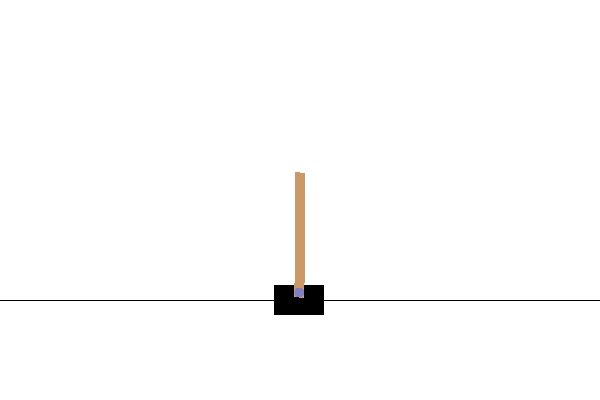
\includegraphics[width=0.5\linewidth]{imgs/random_rollout3.jpg}
	\caption{An example of the visual observation of the cart-pole system.}
	\label{fig:cart-pole}
\end{figure}

\subsection{Imitation Learning \& Uncertainty Estimation with Gaussian Processes}
\subsubsection{State-based Imitation Learning}
When the ground truth states of the cart-pole system are accessible, we use a GP to directly regress the function mapping from states to actions based on the demonstration dataset collected by the expert controller. One of the key benefits of using GP is the learning efficiency, and this is supported by the quantitative results shown in Table \ref{tab:comparison}. The state-based GP controller is able to learn from very few examples (Fig \ref{fig:state-il}:Left), and achieves high accuracies in the state space covered by the training dataset, in the meantime generalizes reasonably well to unseen states (Fig \ref{fig:state-il}:Right).

Furthermore, GP is able to model the epistemic uncertainty (Fig \ref{fig:state-il}:Middle), in which unseen states generally correspond to high uncertainties.

\begin{figure}[ht]
	\centering
	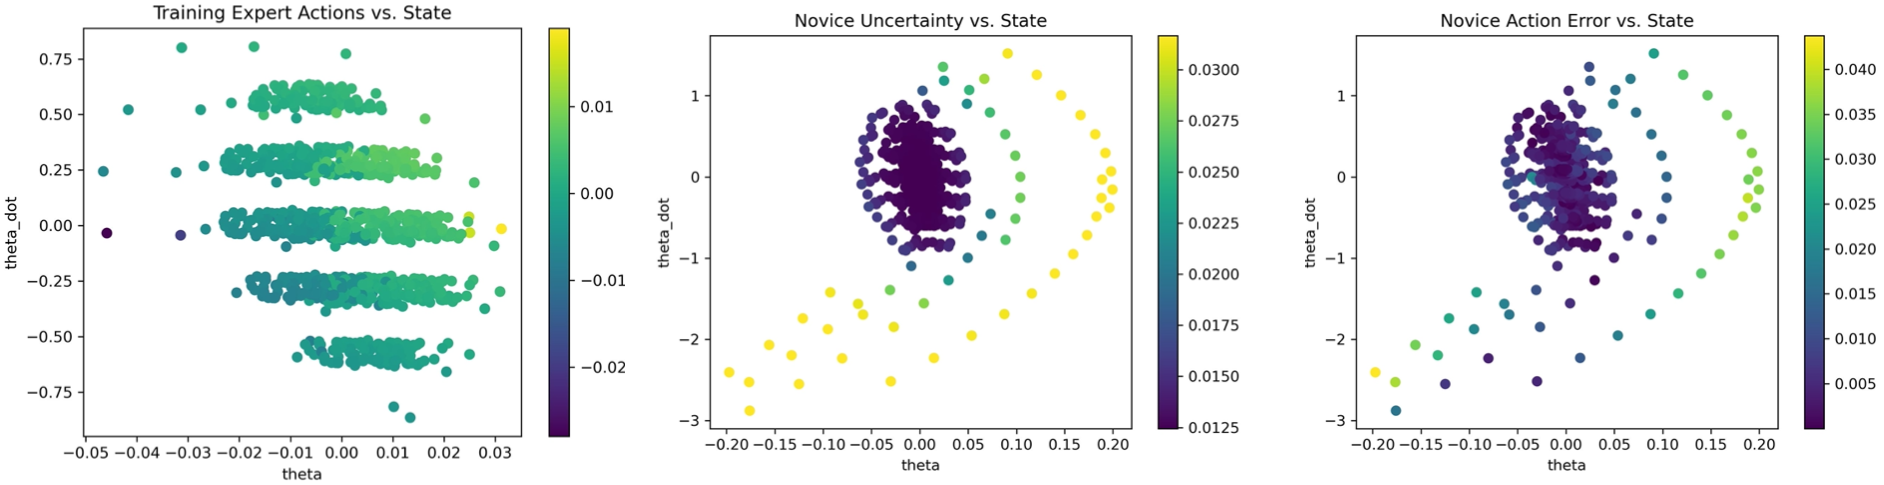
\includegraphics[width=\linewidth]{imgs/state-il.png}
	\caption{State-based imitation learning with GP. Left: visualization of the training demonstration dataset distribution, color represents the expert policy control output (target); Middle: uncertainty estimation from GP on a testing dataset, color represents uncertainty; Right: novice policy control error, color represents the absolute difference between the expert policy action and the novice policy action for a given state.}
	\label{fig:state-il}
\end{figure}

\subsubsection{Visual Imitation Learning} \label{vis-il}
To explore the possibilities of using non-parametric models like GP for high dimensional inputs, we experiment Deep Kernel Learning with a simple imitation learning task. Note that doing visuomotor control is an inherently difficult task in the sense that the model must learn to extract visual features.
We stack two adjacent images together to feed in velocity information.
Compared with state-based IL, visual IL  achieves worse performance despite requiring more training data (Table \ref{tab:comparison}).

We further visualize the uncertainty estimation on the testing dataset in Fig \ref{fig:visual-il}:Middle, and discover that the epistemic uncertainties are not correctly modeled by Deep Kernel Learning, as two observations correspond to very different uncertainties even though their ground truth states are extremely close.

\begin{figure}[ht]
	\centering
	% 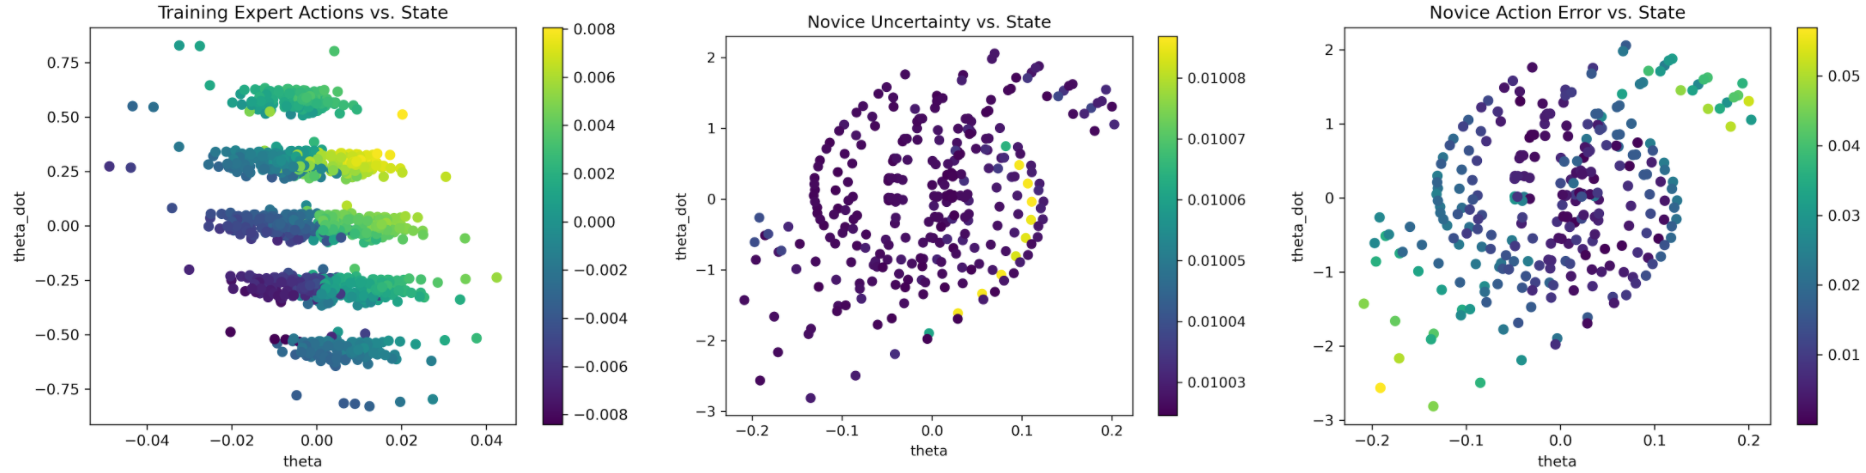
\includegraphics[width=\linewidth]{imgs/visual-il.png}
	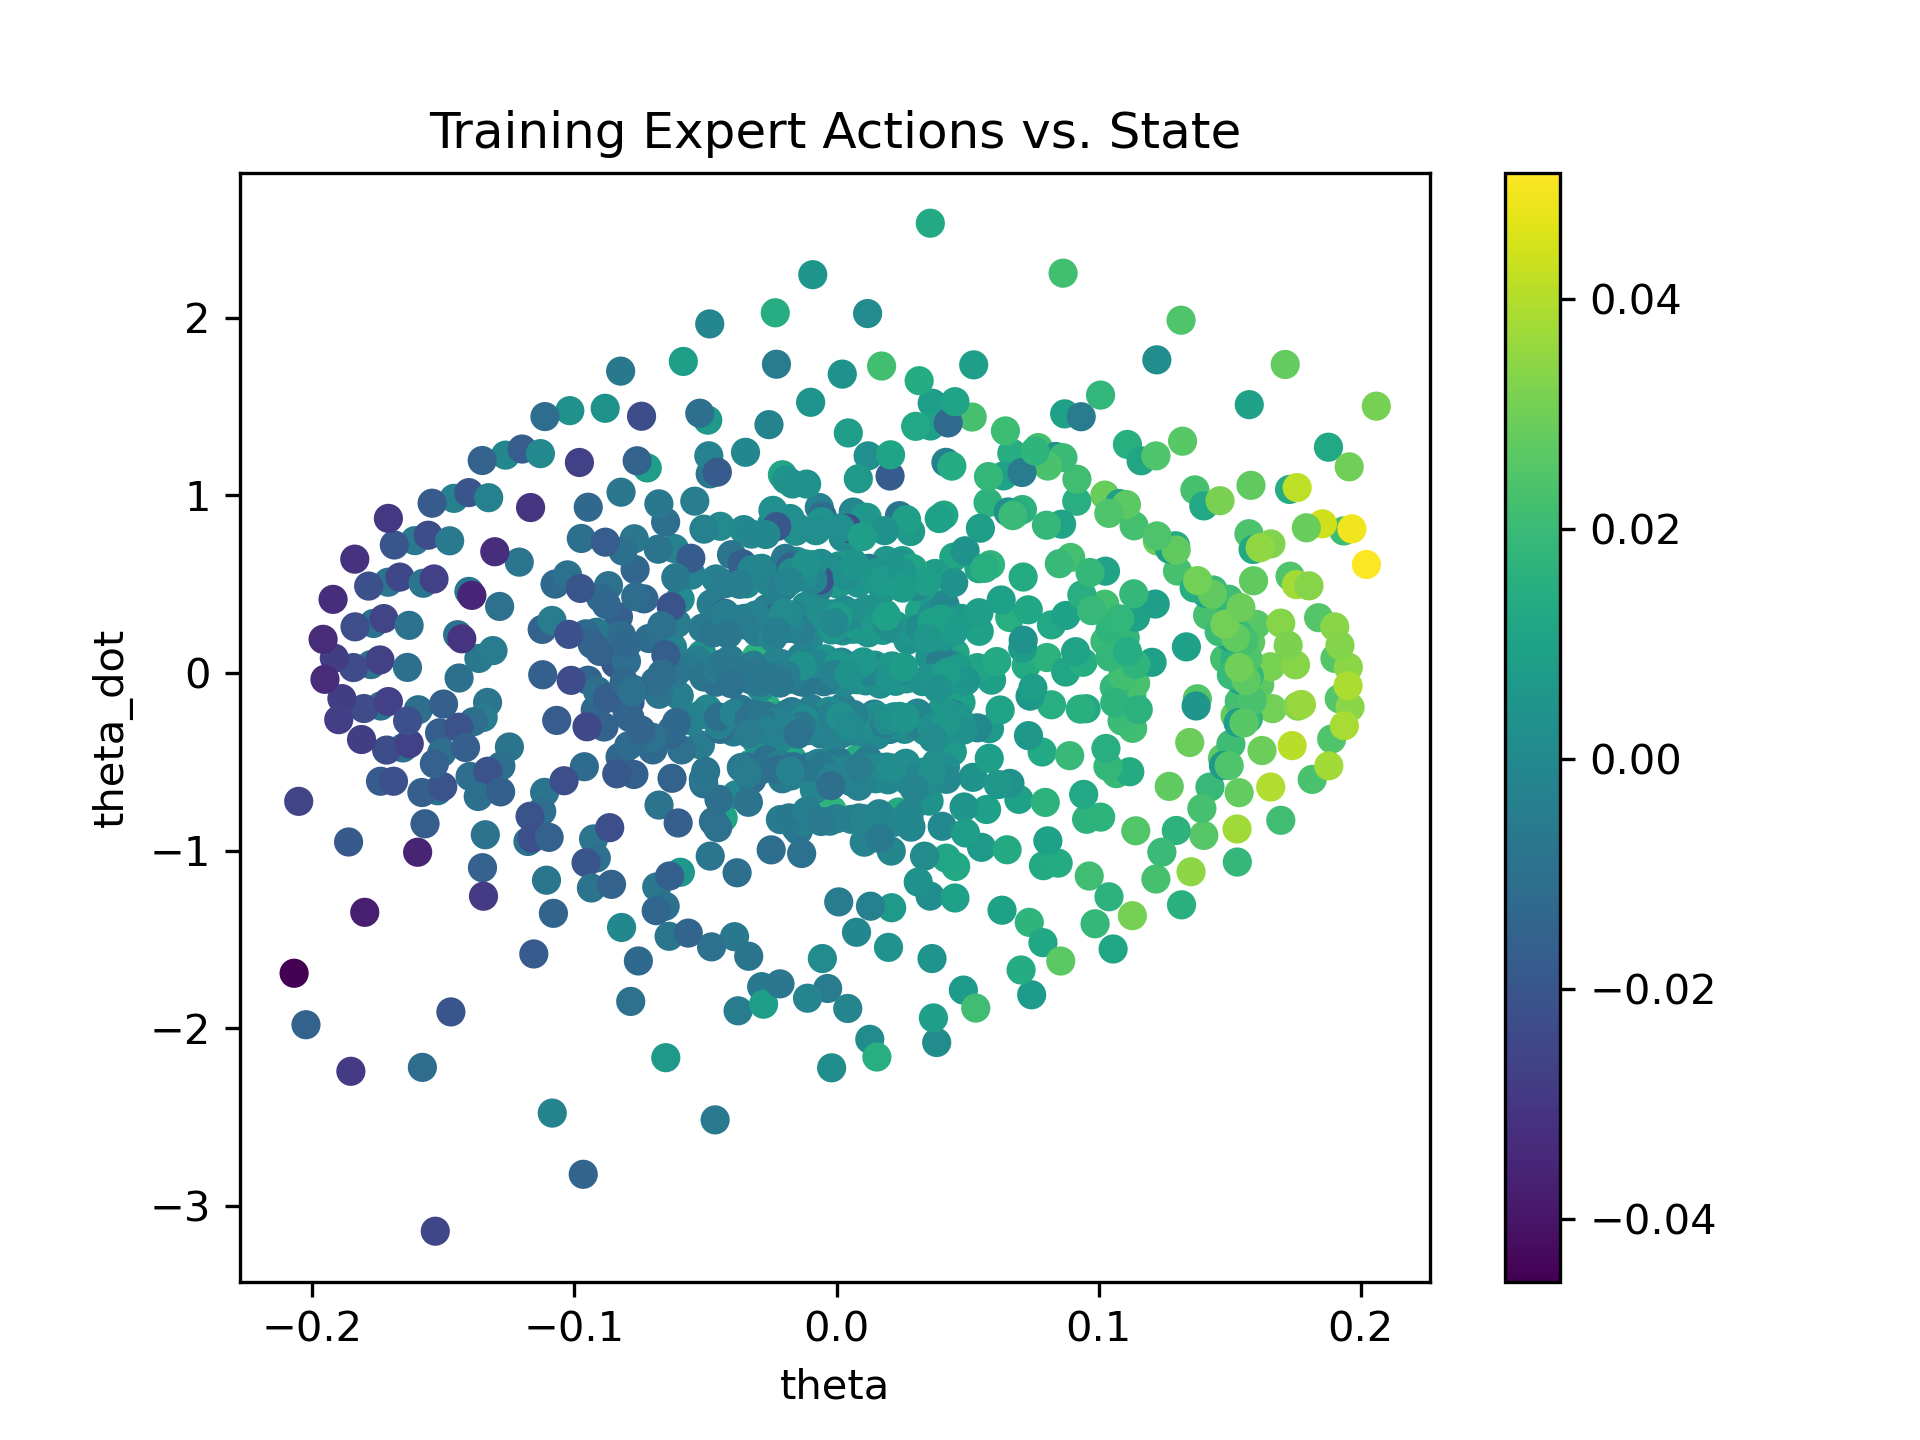
\includegraphics[width=0.32\linewidth]{imgs/expert_data_0.png}
	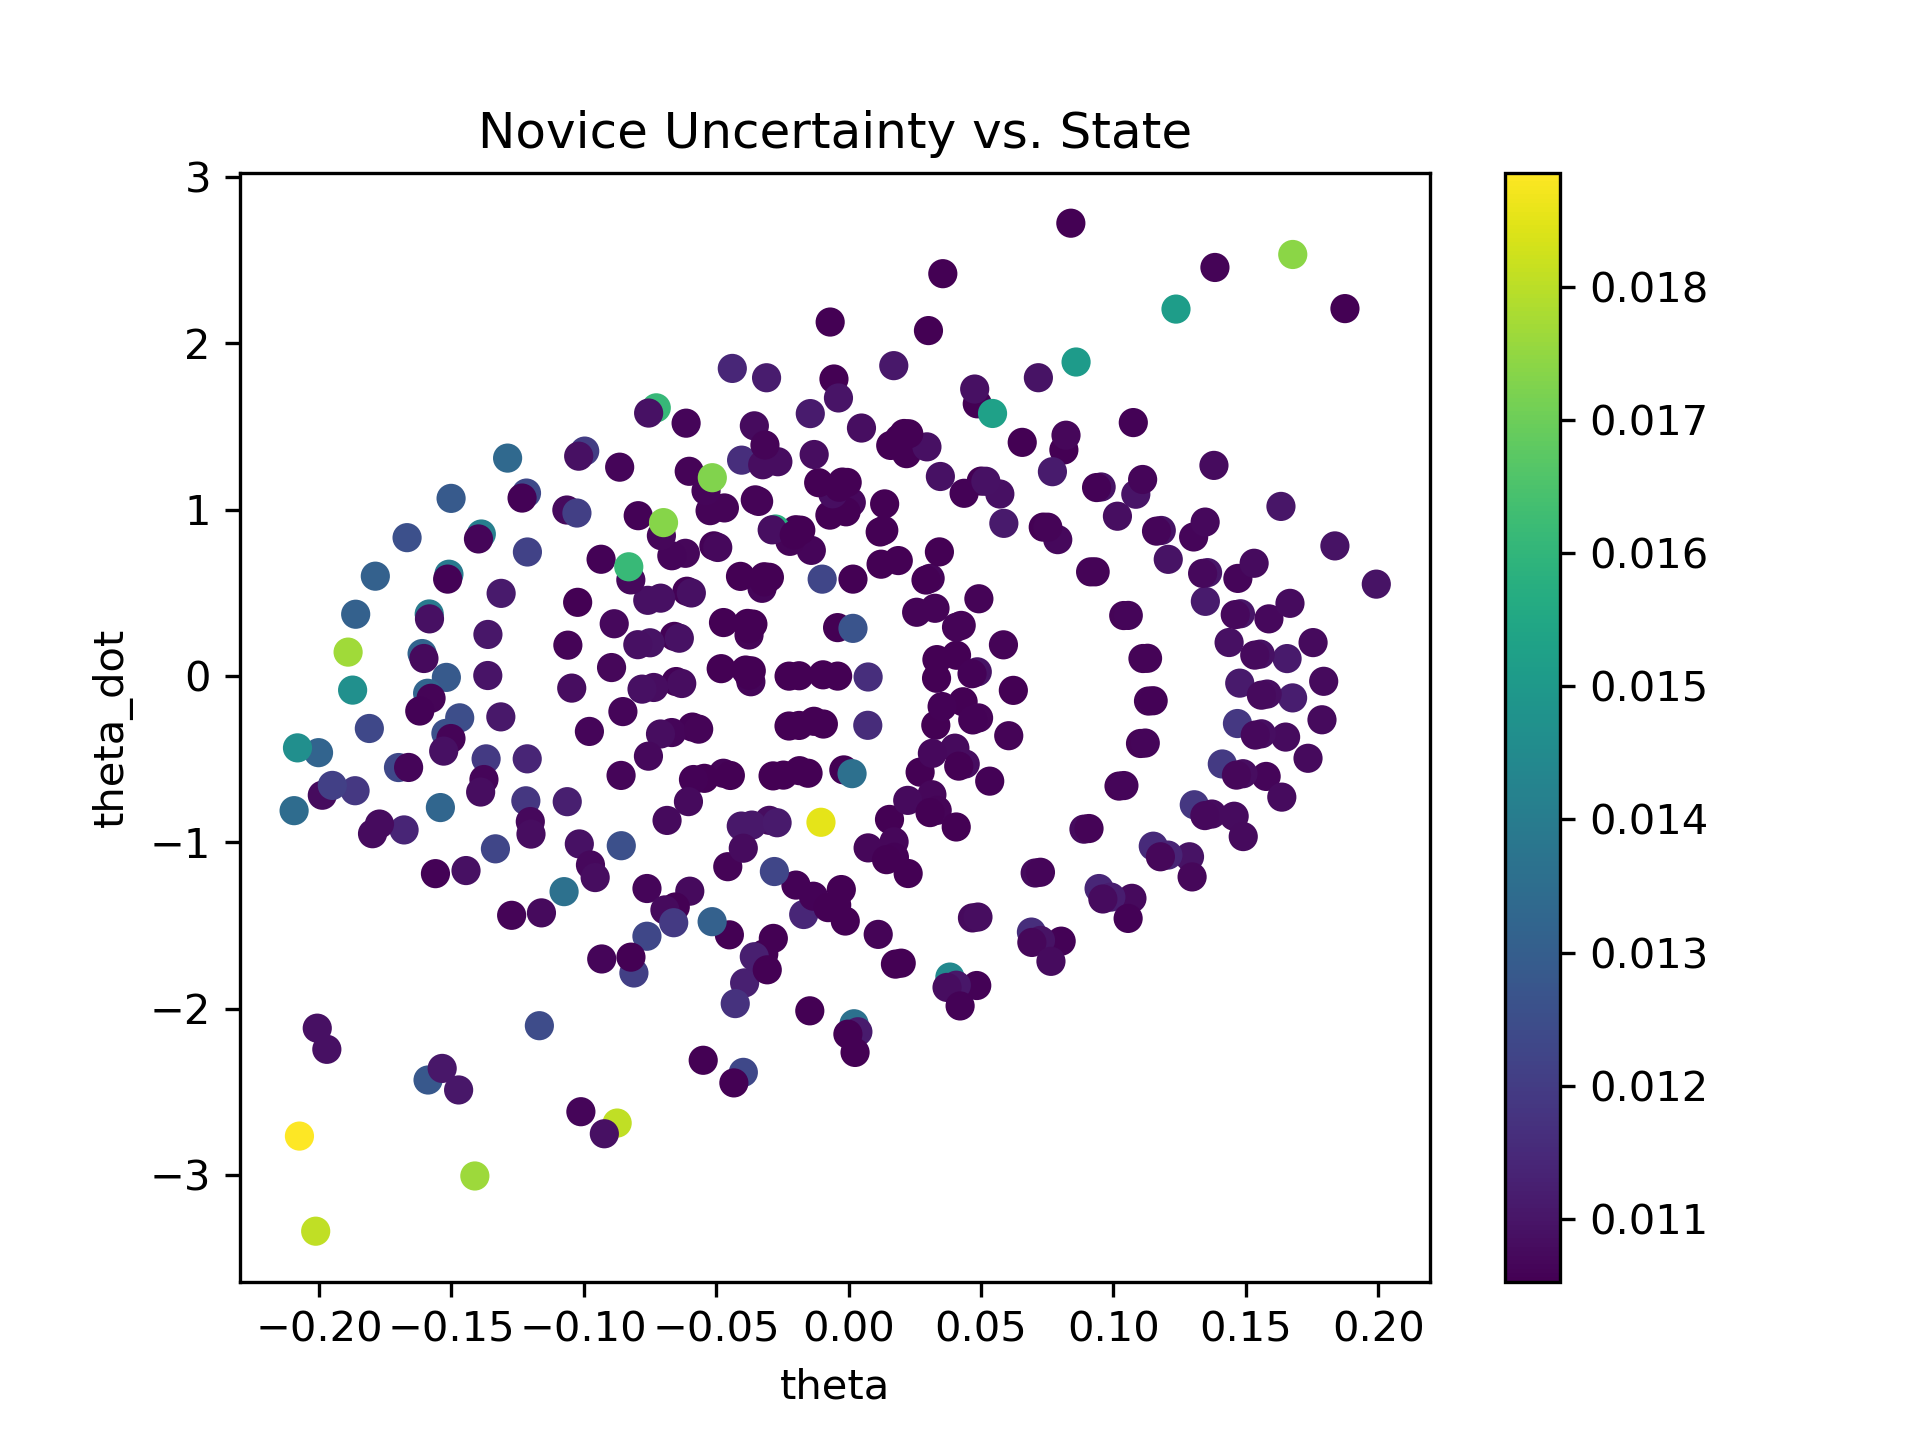
\includegraphics[width=0.32\linewidth]{imgs/novice_uncertainty_0.png}
	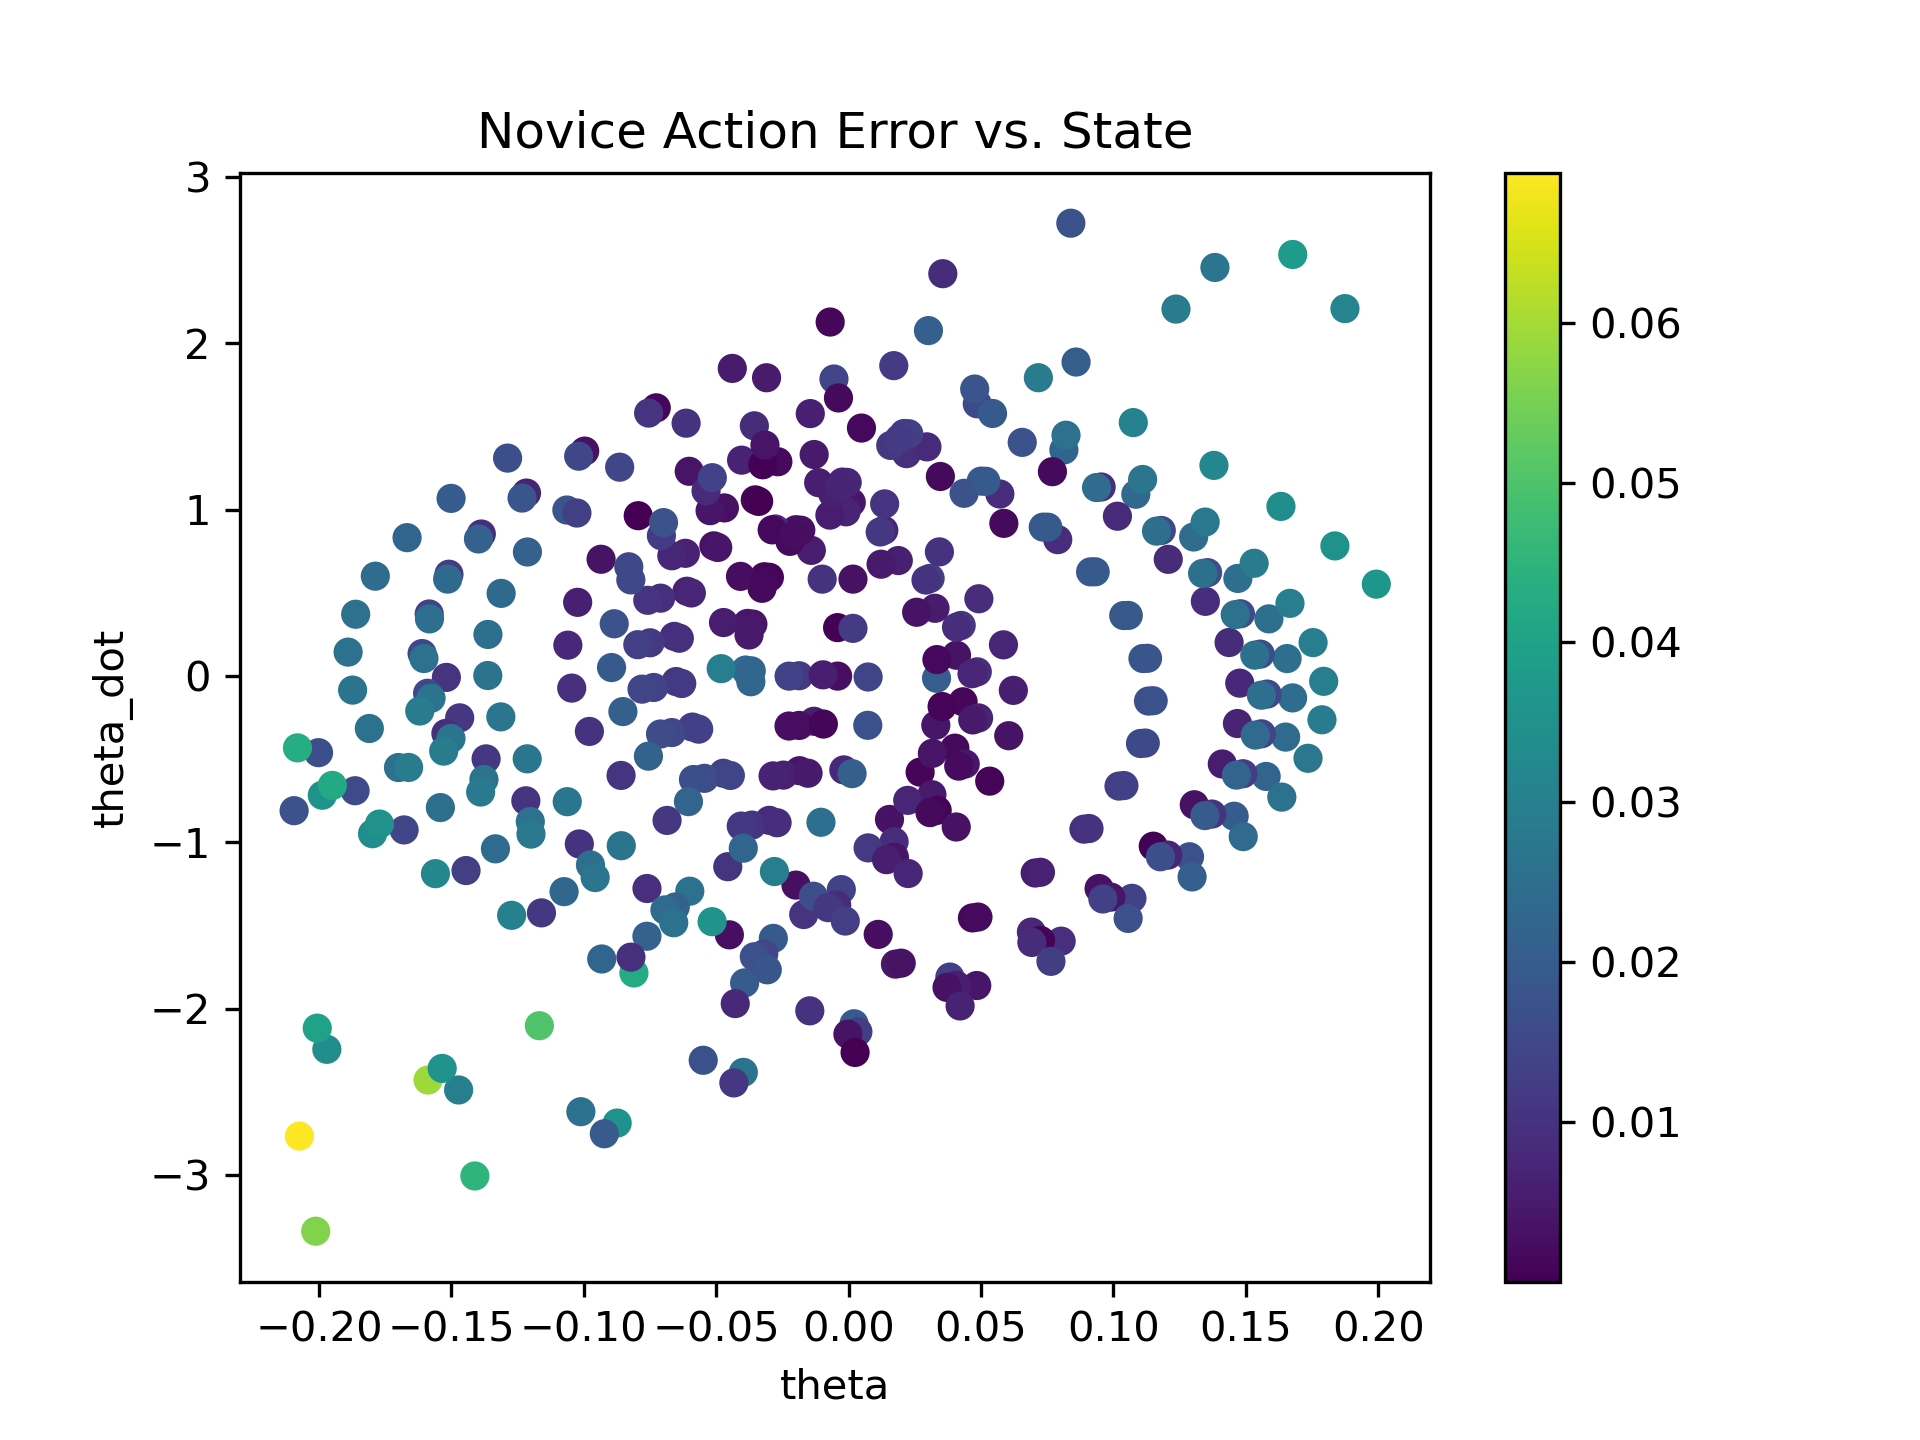
\includegraphics[width=0.32\linewidth]{imgs/novice_error_0.png}
	\caption{Visual imitation learning with GP.}
	\label{fig:visual-il}
\end{figure}

To investigate this issue of uncertainty estimation, following the visualization protocol presented in prior work ``Embed to control'' \cite{watter2015embed}, we set the CNN output latent space to be 2-dimensional, and visualize the mapping between the state space and the latent space as shown in Fig \ref{fig:latent}. Ideally the CNN would be forced to extract the true state information from visual observations. However, the Deep Kernel Learning model fails to discover the underlying structure of the state space. Our hypothesis for this phenomenon is that the image distance does not reflect the actual state distance, thus, without constraints, the model naturally has no clue to learn a structured latent space.

\begin{figure}[ht]
	\centering
	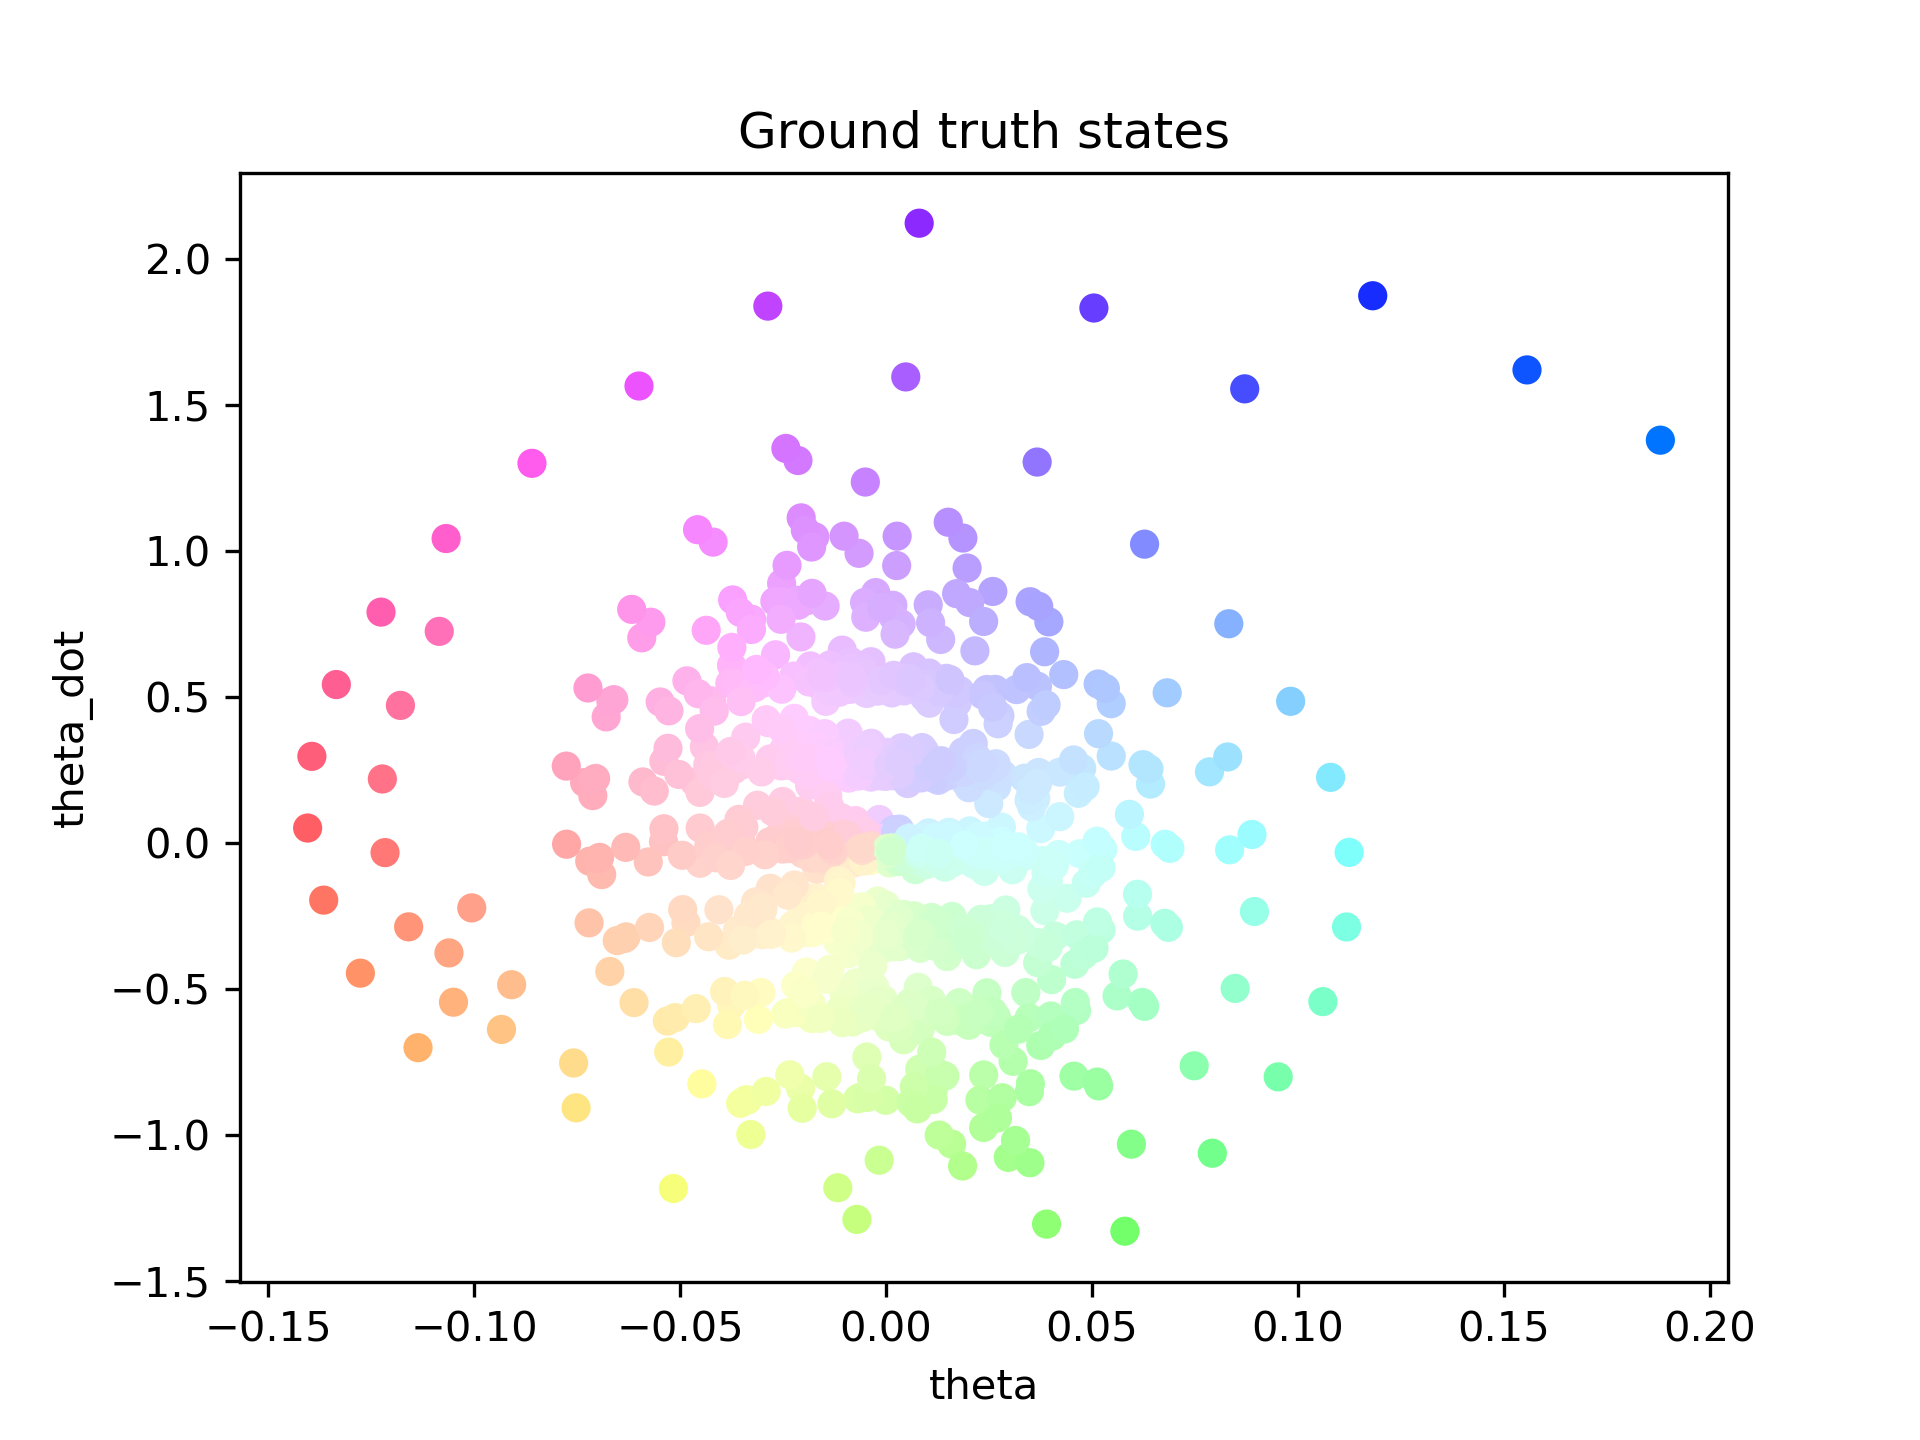
\includegraphics[width=0.4\linewidth]{imgs/latentVis_gt_states_0.png}
	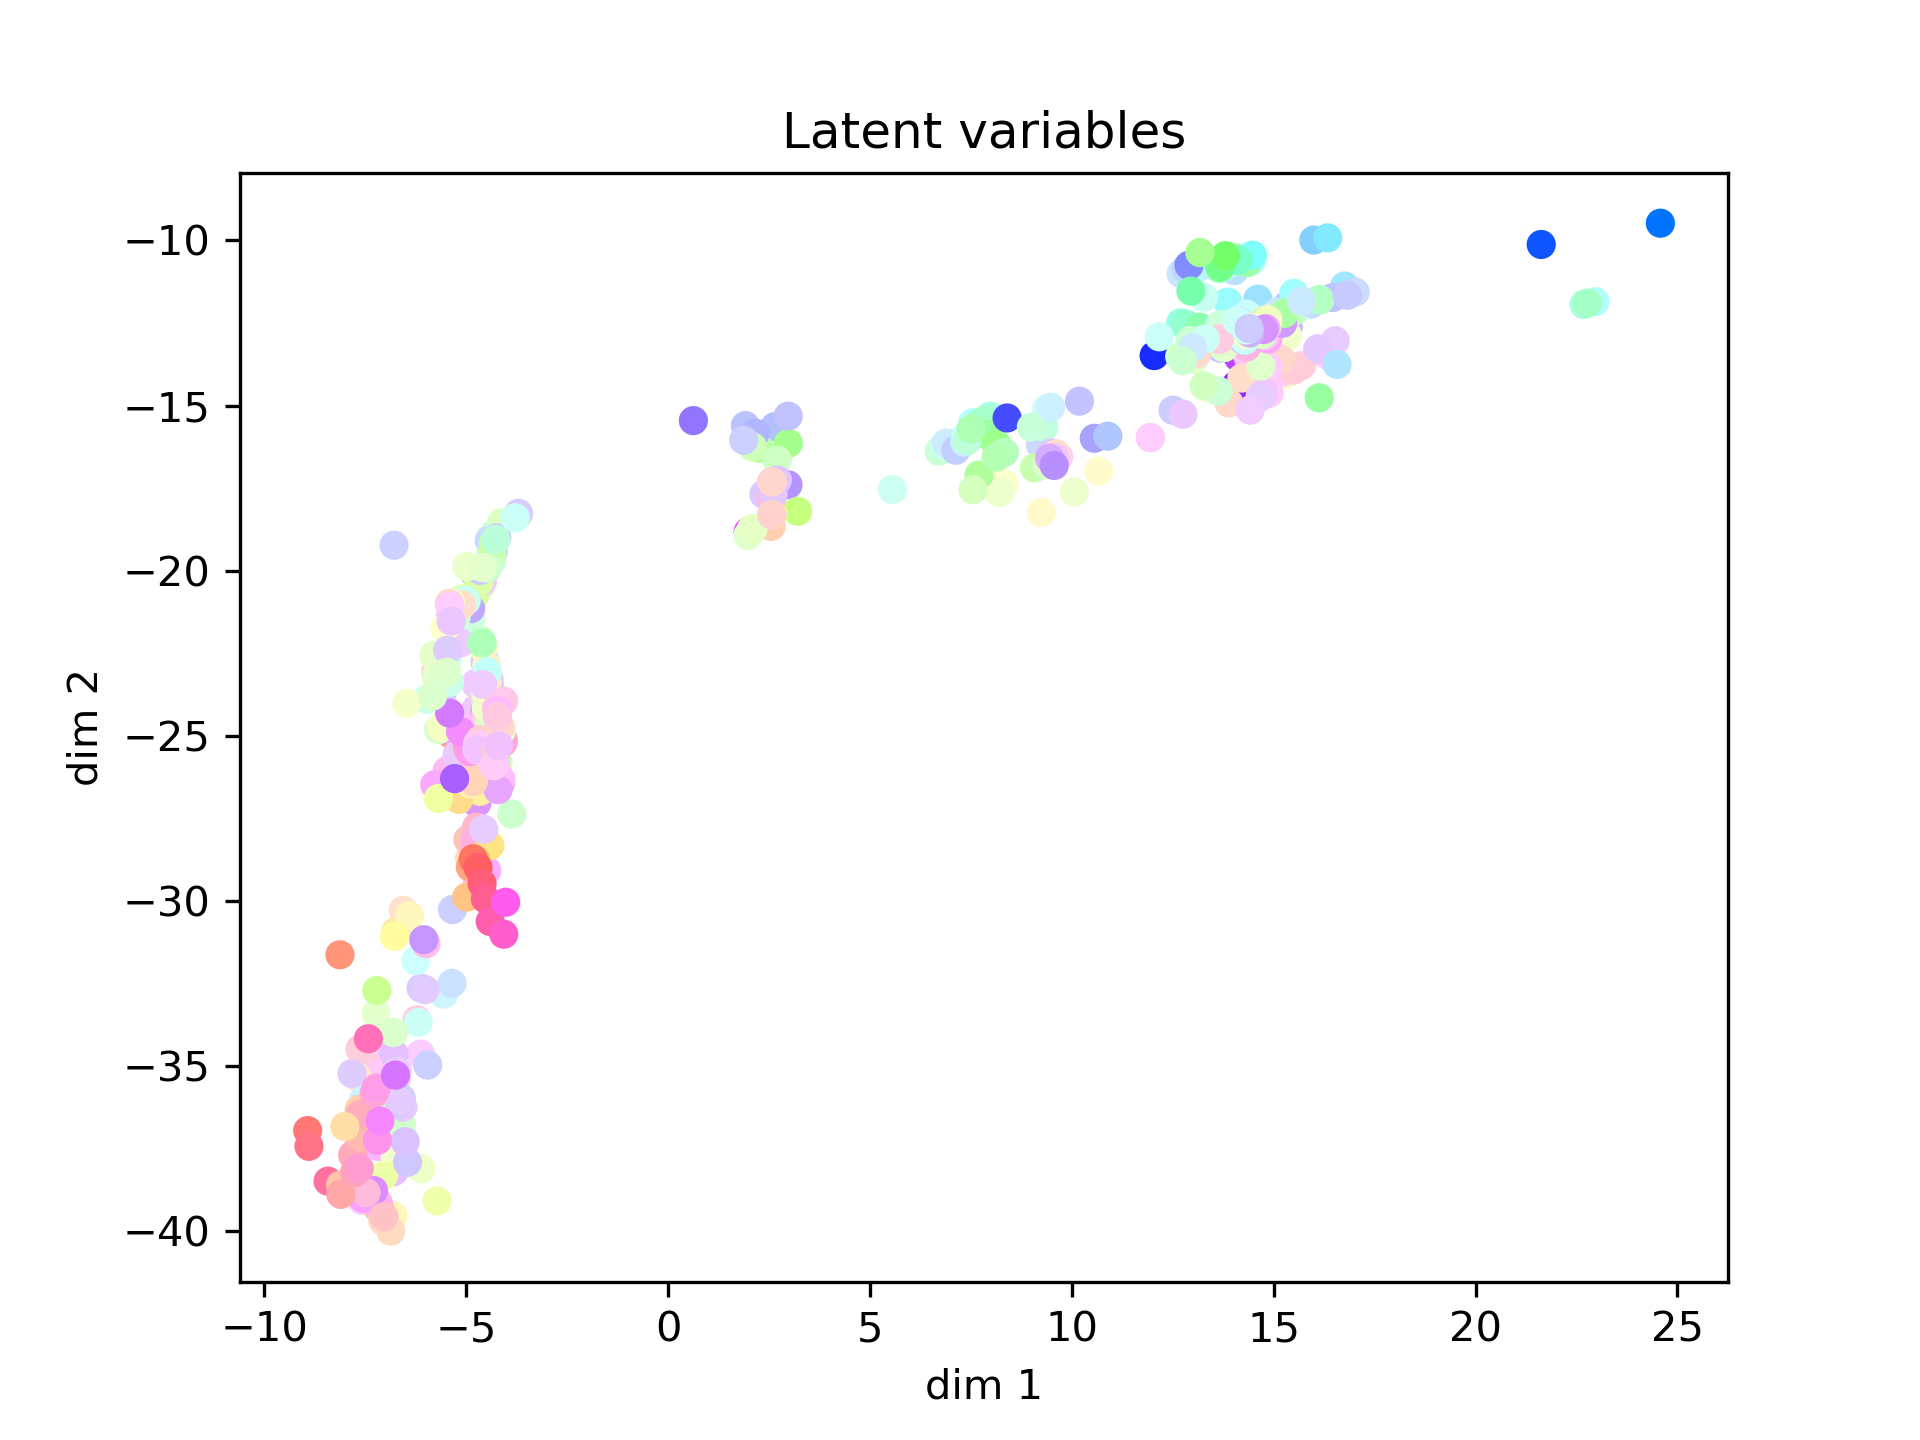
\includegraphics[width=0.4\linewidth]{imgs/latentVis_latents_0.png}
	\caption{Visualization of the latent space learned by the CNN. Left: ground truth states; Right: corresponding learned latent representations. Points in the true state space and the latent space are associated by color.}
	\label{fig:latent}
\end{figure}

\begin{table}[ht]
	\centering
	\begin{tabular}{|l|c|c|}
		\hline
		                                         & Avg Balanced Duration $\uparrow$ & Expert Query Count $\downarrow$ \\
		\hline
		State-based IL                           & 67.1                             & 200.0                           \\
		\hline
		State-based DevDAgger                    & \textbf{74.08}                   & \textbf{178.4}                  \\
		\hhline{|=|=|=|}
		Visual IL                                & \textbf{45.87}                   & 1000.0                          \\
		\hline
		Visual Vanilla DAgger ($\gamma = 0.995$) & 35.6                             & 1000.0                          \\
		\hline
		Visual Vanilla DAgger ($\gamma = 0.999$) & \textbf{45.3}                    & 1000.0                          \\
		\hline
		Visual DevDAgger                         & \textbf{43.15}                   & \textbf{613.3}                  \\
		\hline
	\end{tabular}
	\caption{Quantitative comparison between different approaches in terms of both the average number of time steps during which the inverted pendulum is balanced, and the number of queries made for the expert policy. Each approach is at least tested for 50 trials.}
	\label{tab:comparison}
\end{table}

\subsection{DevDAgger: Uncertainty-based Decision Rule for DAgger}
We further experiment with incorporating uncertainty estimation into online imitation learning algorithm DAgger.

\subsubsection{State-base DevDAgger}
The uncertainty-based decision rule is set as followings: if the predicted uncertainty is larger than $\alpha \sigma_{prior}$ where $\alpha=0.7$, query the expert policy for what action $a$ to take, and aggregate this new state-action pair $(s, a)$ to the current dataset; otherwise, rollout the current novice policy.

With each newly aggregated state-action pair, ideally we would train the GP model again, however, an exact GP model is trained every $30$ data collection steps with the aim to improve runtime efficiency.

The quantitative comparison between the state-based IL and the state-based DevDAgger in Table \ref{tab:comparison} shows that the proposed uncertainty-aware decision rule is able to learn a better policy with fewer expert queries in an online fashion given the ground truth states.

\subsubsection{Visual DevDAgger}
We use the same uncertainty threshold $\alpha$, and experimented with different latent space dimensions $2, 4, 8, 16$.
As discussed in section \ref{vis-il}, the uncertainty estimation of the Deep Kernel Learning model is very problematic due to the unstructured learned latent space. This phenomenon causes the unreasonable behavior of the uncertainty-aware decision rule and fails to improve the performance compared with visual imitation learning (Table \ref{tab:comparison}).

\section{Future Work}
To resolve the issue with the uncertainty estimation of visual GP imitation learning, a structured latent space has to be enforced by adding constraints to the model. A very simple solution would be to train a regression model that predicts the ground truth states from images. We can also use contrastive learning to enforce the structure in the learned latent space. However, both of these two methods rely on supervision, i.e. providing ground truth states as labels for each image.

Without ground truth states as supervision, proposed by \cite{watter2015embed}, we could train a dynamics model in the latent space and force the dynamical model to be linear. As an extension to \cite{watter2015embed}, a more recent work \cite{levine2019prediction} achieves better results in terms of the latent space structure.

\section{Conclusion}
\todo[inline]{Zhihao}

{
	\bibliographystyle{unsrt}
	\bibliography{egbib}
}

\end{document}